\section{Artificial Variables Techniques}
\label{sec:artificial-variables}


\begin{frame}{Artificial Variables Techniques}
  \begin{itemize} \parskip3mm \justifying
  \item<only@1> In the earlier problems, the constraints were of ($\leq$) type (with non-negative right hand sides). The introduction of slack variables readily provided the initial basic feasible solution.
  \item<only@1> In problems where at least one of \alert{the constraints is of ($\geq$) or ($=$) type} we introduce another type of variables called \alert{artificial variables} 
  \item<only@1> These variables are fictitious and have no physical meaning. They assume the role of slack variables of the first iteration, only to be replaced at a later iteration.
  \item<only@2> Thus they are merely a device to get the starting basic feasible solution so that simplex algorithm be applied as usual to get optimal solution.
  \item<only@2> There are two techniques available to solve such problems. They are: 
    \begin{enumerate}
    \item The big \emph{M-method} or \emph{M-technique} or \alert{method of penalties}.
    \item \alert{The two-phase method}.
    \end{enumerate}
  \end{itemize}
\end{frame}

\begin{frame}{The Method of Penalties (Big \emph{M-Method})}
  \begin{description} \justifying \parskip4mm
  \item[Step 1.] Express the linear programming problem in standard form by introducing slack variables.
  \item[Step 2.] Add non-negative variables to the left-hand sides of all the constraints of \emph{initially} ($\geq$) or ($=$) type. These variables are called \alert{artificial variables}. We must get rid of these variables and must not allow them to appear in the final solution. To achieve this, these variables are assigned a very large per unit penalty in the objective function. This penalty is designated by \alert{$-M$ for maximization problems and $+M$ for minimization problems}, where $M > 0$.
  \item[Step 3.] Solve the modified linear programming problem by the simplex method.
  \end{description}
\end{frame}

\begin{frame}{The Method of Penalties (Big \emph{M-Method})}
  While making iterations, using the simplex method, one of the following three cases may arise:
  \begin{enumerate} \justifying \parskip5mm
  \item If \alert{no artificial variable remains in the basis} and the optimality condition is satisfied, then \alert{the solution is an optimal feasible solution the the given problem}.
  \item If at least one \alert{artificial variable appears in the basis at zero} level (with zero value in \emph{b}-column) and the optimality condition is satisfied, then \alert{the solution is optimal feasible (though degenerate)} solution to the given problem.
  \item If at least \alert{one artificial variable appears in the basis at a non-zero level} (with positive value in \emph{b}-column) and the optimality condition is satisfied, then \alert{the original problem has no feasible solution}.
  \end{enumerate}
\end{frame}

\begin{frame}{Method of Penalties. An Example}{}
      Food $X$ contains 6 units of vitamin A per gram and 7 units of vitamin B per gram and costs \$12  per gram. Food $Y$ contains 8 units of vitamin A per gram and 12 units of vitamin B per gram and costs \$20  per gram. The daily minimum requirement of vitamin A and vitamin B is 100 units and 120 units respectively. Find the minimum cost of product mix by the simplex method.


      \begin{block}{The Model} \justifying
          \[\min Z = 12x_1 + 20x_2\]

          {\centering
            s.t.

            \sysdelim..%
            \sysalign{r,r}%
            \systeme[x_1x_2]{%
              6x_1 + 8x_2   \geq 100,
              7x_1 + 12x_2 \geq    120
            }% systeme

            $    x_1, x_2  \geq 0$
            \par}
      \end{block}
\end{frame}

\begin{frame}{Method of Penalties. An Example}{}


  \begin{block}<only@1>{Model}
\[     \min Z = 12x_1 + 20x_2\]

{\centering
  s.t.

  \sysdelim..%
  \sysalign{r,r}%
  \systeme[x_1x_2]{%
      6x_1 + 8x_2   \geq 100,
    7x_1 + 12x_2 \geq    120
}% systeme

$    x_1, x_2  \geq 0$
\par}
  \end{block}
\begin{block}<only@1,2>{Step 1. Express The Problem in Standard Form} \justifying

  \[\min Z = 12x_1 + 20x_2 + 0s_1 + 0s_2\]

  {\centering
    s.t.

    \sysdelim..%
  \sysalign{r,r}%
  \systeme[x_1x_2s_1s_2]{%
      6x_1 + 8x_2 - s_1  = 100,
    7x_1 + 12x_2 - s_2   = 120
}% systeme

$    x_1, x_2, s_1, s_2  \geq 0$
\par}
\end{block}

\begin{block}<only@2>{Step 2. Find initial basic feasible solution} \justifying
    \[\min Z = 12x_1 + 20x_2 + 0s_1 + 0s_2 +MA_1 + MA_2\]

    {\centering
      s.t.

      \sysdelim..%
  \sysalign{r,r}%
  \systeme[x_1x_2s_1s_2A_1A_2]{%
      6x_1 + 8x_2 - s_1 + A_1 = 100,
    7x_1 + 12x_2 - s_2   + A_2= 120
}% systeme

$    x_1, x_2, s_1, s_2, A_1, A_2   \geq 0$
\par}
\end{block}

\begin{block}<only@3>{Step 3. Perform optimality test.} \justifying
  {\centering
    \scalebox{0.8}{%
      \begin{tabular}{cccccccccc}
        \toprule
      $\min$ &$c_j$&12&20&0&0&$M$&$M$&& \\
      $c_B$&Basis&$x_1$&\cellcolor{yellow}$x_2$&$s_1$&$s_2$&$A_1$&$A_2$&$b$&$\theta$\\
      \midrule
      $M$&$A_1$&6&8&-1&0&1&0&100&$\nicefrac{100}{8}=25/2$\\
      $M$&\cellcolor{yellow}$A_2$&7&\cellcolor{orange}12&0&-1&0&1&120&$\nicefrac{120}{12}=10$ \textrightarrow\\
      \midrule
           &$Z_j$&$13M$&$20M$&$-M$&$-M$&$M$&$M$&\cellcolor{red!20}$220M$&\\
           &$c_j - Z_j$&$12 - 13M$&$20-20M$&$M$&$M$&0&0&&\\
        \bottomrule
           &&&\textuparrow&&&&&&\\
           &&&K&&&&&&\\
    \end{tabular}
    }%
  \par}
\end{block}

\begin{block}<only@4>{Step 4. Iterate towards on optimal solution.} \justifying
  {\centering
    \scalebox{0.7}{%
      \begin{tabular}{ccccccccc}
        \toprule
      $\min$ &$c_j$&12&20&0&0&$M$&& \\
      $c_B$&Basis&\cellcolor{yellow}$x_1$&$x_2$&$s_1$&$s_2$&$A_1$&$b$&$\theta$\\
      \midrule
      $M$&\cellcolor{yellow}$A_1$&\cellcolor{orange}\nicefrac{4}{3}&0&-1&\nicefrac{2}{3}&1&20&15\textrightarrow\\
      20&$x_2$&\nicefrac{7}{12}&1&0&\nicefrac{-1}{12}&0&10&\nicefrac{120}{7} \\
      \midrule
           &$Z_j$&$\frac{35}{3} + \frac{4}{3}M$&$20$&$-M$&$-\frac{5}{3} + \frac{2}{3}M$&$M$&\cellcolor{red!20}$200 + 20M$&\\[3mm]
           &$c_j - Z_j$&$\frac{1}{3} - \frac{4}{3}M$&0&$M$&$\frac{5}{3} - \frac{2}{3}M$&0&&\\
        \bottomrule
           &&\textuparrow K&&&&&&\\
           % &&&K&&&&&\\
    \end{tabular}
    }%
    \par}

  \begin{columns}
    \column{0.6\textwidth}
        \scalebox{0.7}{%
      \begin{tabular}{ccccccc}
        \toprule
      $\min$ &$c_j$&12&20&0&0& \\
      $c_B$&Basis&$x_1$&$x_2$&$s_1$&$s_2$&$b$\\
      \midrule
      12&$x_1$&1&0&-\nicefrac{3}{4}&\nicefrac{1}{2}&15\\
      20&$x_2$&0&1&\nicefrac{7}{16}&-\nicefrac{3}{8}&\nicefrac{5}{4} \\
      \midrule
           &$Z_j$&12&20&-\nicefrac{1}{4}&-\nicefrac{3}{2}&205\\
           &$c_j - Z_j$&\cellcolor{blue!30}0&\cellcolor{blue!30}0&\cellcolor{blue!30}\nicefrac{1}{4}&\cellcolor{blue!30}\nicefrac{3}{2}&\\
        \bottomrule
    \end{tabular}
  }%
  \column{0.4\textwidth}
  Optimal solution found is
  \begin{flalign*}
    x_1 & = 15\\
    x_2 & = \frac{5}{4}\\
    Z_{\min} &= 205
  \end{flalign*}
  \end{columns}

\end{block}

\end{frame}




\begin{frame}{Method of Penalties. An Example}{}

  \begin{onlyenv}<1>
    \begin{columns}
      \column{0.3\textwidth}

        \[ \max Z = 2x_1 + 3x_2 \]

        {\centering
          subject to

          \sysdelim..\sysalign{r,r}%
          \systeme[x_1x_2]%
          {
            x_1 + x_2  \leq 30,
        x_2  \geq 3,
        x_2  \leq 12,
        x_1 - x_2  \geq 0,
        x_1   \leq 20 
      }

      \vspace{5mm}
              $x_1, x_2  \geq 0$
        \par}

      \column{0.7\textwidth}
        \[\max Z = 2x_1 + 3x_2 - MA_2 \]

        {\centering
          subject to

\sysdelim..\sysalign{r,r}%
          \systeme[x_1x_2s_1s_2s_3s_4A_2]%
          {
            x_1 + x_2 + s_1   = 30,
            x_2  - s_2  + A_2 = 3,
            x_2  + s_3 = 12,
            -x_1 + x_2 + s_4  =  0,
            x_1  + s_5 = 20
          }

          \vspace{5mm}
      $x_1, x_2, s_1, s_2, s_3, s_4, s_5, A_2  \geq 0$
    \par}

    \end{columns}
  \end{onlyenv}

  \begin{onlyenv}<2>

    \[ \max Z = 2x_1 + 3x_2 +0s_1 - 0s_2 + 0s_3 + 0s_4 + 0s_5 - MA_2 \]

    {\centering
      subject to

      \sysdelim..%
      \sysalign{r,r}%
      \systeme[x_1x_2s_1s_2s_3s_4s_5A_2]
      {%
      x_1 + x_2 + s_1 = 30,
      x_2  - s_2  + A_2 = 3,
      x_2  + s_3 = 12,
      -x_1 + x_2 + s_4  =  0,
      x_1  + s_5 = 20
    }

    \vspace{5mm}
    $x_1, x_2, s_1, s_2, s_3, s_4, s_5, A_2  \geq 0$
  \par}
  \end{onlyenv}
\end{frame}

\begin{frame}{Método de Penalización. Ejemplo.}{}
  Tabla Simplex Inicial

  {\centering
    \begin{tabular}{rc|rr|rrrrrr|r}
      & $\max$ & 2 & 3 & 0 & $-M$ & 0 & 0 & 0 & 0 &  \\
      \toprule
      $\mathbf{Cb}$ & \textbf{basis} & $x_1$ & $x_2$ & $s_1$ & $A_2$ & $s_3$ & $s_4$ & $s_5$ & $s_2$ & RHS \\
      \toprule
      0 & $s_1$ & 1 & 1 & 1 & 0 & 0 & 0 & 0 & 0 & 30 \\
      $-M$ & $A_2$ & 0 & 1 & 0 & 1 & 0 & 0 & 0 & -1 & 3 \\
      0 & $s_3$ & 0 & 1 & 0 & 0 & 1 & 0 & 0 & 0 & 12 \\
      0 & $s_4$ & -1 & 1 & 0 & 0 & 0 & 1 & 0 & 0 & 0 \\
      0 & $s_5$ & 1 & 0 & 0 & 0 & 0 & 0 & 1 & 0 & 20\\
      \bottomrule
    \end{tabular}
    \par}

\end{frame}

\begin{frame}{Método de Penalización. Ejemplo.}{}
  {\centering
    \scalebox{0.85}{%
      \begin{tabular}{rc|rrrrrrrr|rr}
        & $\max $ & 2 & 3 & 0 & $-M$ & 0 & 0 & 0 & 0 &  &  \\
        \toprule
        $\mathbf{C_b}$ & \textbf{basis} & $x_1$ & $x_2$ & $s_1$ & $A_2$ & $s_3$ & $s_4$ & $s_5$ & $s_2$ & RHS & ratios \\
        \toprule
        \only<1>{%
        0 & $s_1$ & 1 & 1 & 1 & 0 & 0 & 0 & 0 & 0 & 30 & 30 \\
        $-M$ & $A_2$ & 0 & 1 & 0 & 1 & 0 & 0 & 0 & -1 & 3 & 3 \\
        0 & $s_3$ & 0 & 1 & 0 & 0 & 1 & 0 & 0 & 0 & 12 & 12 \\
        0 & $s_4$ & -1 & \cellcolor{yellow}{1} & 0 & 0 & 0 & 1 & 0 & 0 & 0 & 0 \\
        0 & $s_5$ & 1 & 0 & 0 & 0 & 0 & 0 & 1 & 0 & 20 & \#DIV/0! \\
        \midrule
        Iter & $Z_j$ & 0 & $-M$ & 0 & $-M$ & 0 & 0 & 0 & $M$ & $-3M$ &  \\
        1 & $c_j - Z_j$ & 2 & $M+3$ & 0 & 0 & 0 & 0 & 0 & $-M$ &  & \\
        } % only
        \only<2>{%
        0 & $s_1$ & 2 & 0 & 1 & 0 & 0 & -1 & 0 & 0 & 30 &  \\
        $-M$ & $A_2$ & 1 & 0 & 0 & 1 & 0 & -1 & 0 & -1 & 3 &  \\
        0 & $s_3$ & 1 & 0 & 0 & 0 & 1 & -1 & 0 & 0 & 12 &  \\
        3 & $x_2$ & -1 & \cellcolor{yellow}1 & 0 & 0 & 0 & 1 & 0 & 0 & 0 &  \\
        0 & $s_5$ & 1 & 0 & 0 & 0 & 0 & 0 & 1 & 0 & 20 &  \\
        \midrule
        Iter & $Z_j$ & $-M-3$ & 3 & 0 & $-M$ & 0 & $M+3$ & 0 & $M$ & $-3M$ &  \\
        1 & $c_j - Z_j$ & $M+5$ & 0 & 0 & 0 & 0 & $-M-3$ & 0 & $-M$ &  & \\
        } % only
        \only<3>{%
        0 & $s_1$ & 2 & 0 & 1 & 0 & 0 & -1 & 0 & 0 & 30 & 15 \\
        $-M$ & $A_2$ & \cellcolor{yellow}1 & 0 & 0 & 1 & 0 & -1 & 0 & -1 & 3 & 3 \\
        0 & $s_3$ & 1 & 0 & 0 & 0 & 1 & -1 & 0 & 0 & 12 & 12 \\
        3 & $x_2$ & -1 & 1 & 0 & 0 & 0 & 1 & 0 & 0 & 0 & -0 \\
        0 & $s_5$ & 1 & 0 & 0 & 0 & 0 & 0 & 1 & 0 & 20 & 20 \\
        \midrule
        Iter & $Z_j$ & $-M-3$ & 3 & 0 & $-M$ & 0 & $+M$ & 0 & $+M$ & $-3M$ &  \\
        2 & $c_j - Z_j$ & $M + 5$ & 0 & 0 & 0 & 0 & $-M-3$ & 0 & $-M$ &  & 
                                                                           } % only
                                                                           \only<4>{%
                                                                           0 & $s_1$ & 0 & 0 & 1 & -2 & 0 & 1 & 0 & 2 & 24 &  \\
        2 & $x_1$ & \cellcolor{yellow}1 & 0 & 0 & 1 & 0 & -1 & 0 & -1 & 3 &  \\
        0 & $s_3$ & 0 & 0 & 0 & -1 & 1 & 0 & 0 & 1 & 9 &  \\
        3 & $x_2$ & 0 & 1 & 0 & 1 & 0 & 0 & 0 & -1 & 3 &  \\
        0 & $s_5$ & 0 & 0 & 0 & -1 & 0 & 1 & 1 & 1 & 17 &  \\
        \midrule
        Iter & $Z_j$ & 2 & 3 & 0 & 5 & 0 & -2 & 0 & -5 & 15 &  \\
        2 & $c_j - Z_j$ & 0 & 0 & 0 & $-M-5$ & 0 & 2 & 0 & 5 &  & 
                                                                  } % only
                                                                  \only<5>{%
                                                                  0 & $s_1$ & 0 & 0 & 1 & -2 & 0 & 1 & 0 & 2 & 24 & 12 \\
        2 & $x_1$ & 1 & 0 & 0 & 1 & 0 & -1 & 0 & -1 & 3 & -3 \\
        0 & $s_3$ & 0 & 0 & 0 & -1 & 1 & 0 & 0 & \cellcolor{yellow}1 & 9 & 9 \\
        3 & $x_2$ & 0 & 1 & 0 & 1 & 0 & 0 & 0 & -1 & 3 & -3 \\
        0 & $s_5$ & 0 & 0 & 0 & -1 & 0 & 1 & 1 & 1 & 17 & 17 \\
        \midrule
        Iter & $Z_j$ & 2 & 3 & 0 & 5 & 0 & -2 & 0 & -5 & 15 &  \\
        3 & $c_j - Z_j$ & 0 & 0 & 0 & $-M-5$ & 0 & 2 & 0 & 5 &  & 
                                                                  } % only
                                                                  \only<6>{%
                                                                  0 & $s_1$ & 0 & 0 & 1 & 0 & -2 & 1 & 0 & 0 & 6 &  \\
        2 & $x_1$ & 1 & 0 & 0 & 0 & 1 & -1 & 0 & 0 & 12 &  \\
        0 & $s_2$ & 0 & 0 & 0 & -1 & 1 & 0 & 0 & \cellcolor{yellow}1 & 9 &  \\
        3 & $x_2$ & 0 & 1 & 0 & 0 & 1 & 0 & 0 & 0 & 12 &  \\
        0 & $s_5$ & 0 & 0 & 0 & 0 & -1 & 1 & 1 & 0 & 8 &  \\
        \midrule
        Iter & $Z_j$ & 2 & 3 & 0 & 0 & 5 & -2 & 0 & 0 & 60 &  \\
        3 & $c_j - Z_j$ & 0 & 0 & 0 & $-M$ & -5 & 2 & 0 & 0 &  & 
                                                                 } % only
                                                                 \only<7>{%
                                                                 0 & $s_1$ & 0 & 0 & 1 & 0 & -2 & \cellcolor{yellow}1 & 0 & 0 & 6 & 6 \\
        2 & $x_1$ & 1 & 0 & 0 & 0 & 1 & -1 & 0 & 0 & 12 & -12 \\
        0 & $s_2$ & 0 & 0 & 0 & -1 & 1 & 0 & 0 & 1 & 9 & \#DIV/0! \\
        3 & $x_2$ & 0 & 1 & 0 & 0 & 1 & 0 & 0 & 0 & 12 & \#DIV/0! \\
        0 & $s_5$ & 0 & 0 & 0 & 0 & -1 & 1 & 1 & 0 & 8 & 8 \\
        \midrule
        Iter & $Z_j$ & 2 & 3 & 0 & 0 & 5 & -2 & 0 & 0 & 60 &  \\
        4 & $c_j - Z_j$ & 0 & 0 & 0 & $-M$ & -5 & 2 & 0 & 0 &  & 
                                                                 } % only
                                                                 \only<8>{%
                                                                 0 & $s_4$ & 0 & 0 & 1 & 0 & -2 & \cellcolor{yellow}1 & 0 & 0 & 6 &  \\
        2 & $x_1$ & 1 & 0 & 1 & 0 & -1 & 0 & 0 & 0 & 18 &  \\
        0 & $s_2$ & 0 & 0 & 0 & -1 & 1 & 0 & 0 & 1 & 9 &  \\
        3 & $x_2$ & 0 & 1 & 0 & 0 & 1 & 0 & 0 & 0 & 12 &  \\
        0 & $s_5$ & 0 & 0 & -1 & 0 & 1 & 0 & 1 & 0 & 2 &  \\
        \midrule
        Iter & $Z_j$ & 2 & 3 & 2 & 0 & 1 & 0 & 0 & 0 & 72 &  \\
        4 & $c_j - Z_j$ & 0 & 0 & -2 & $-M$ & -1 & 0 & 0 & 0 &\textbf{END}  & 
                                                                              } % only
                                                                              % \bottomrule
      \end{tabular}
    } % scalebox
    \par}
    
    % \begin{onlyenv}<9>
    %   {\centering
    %   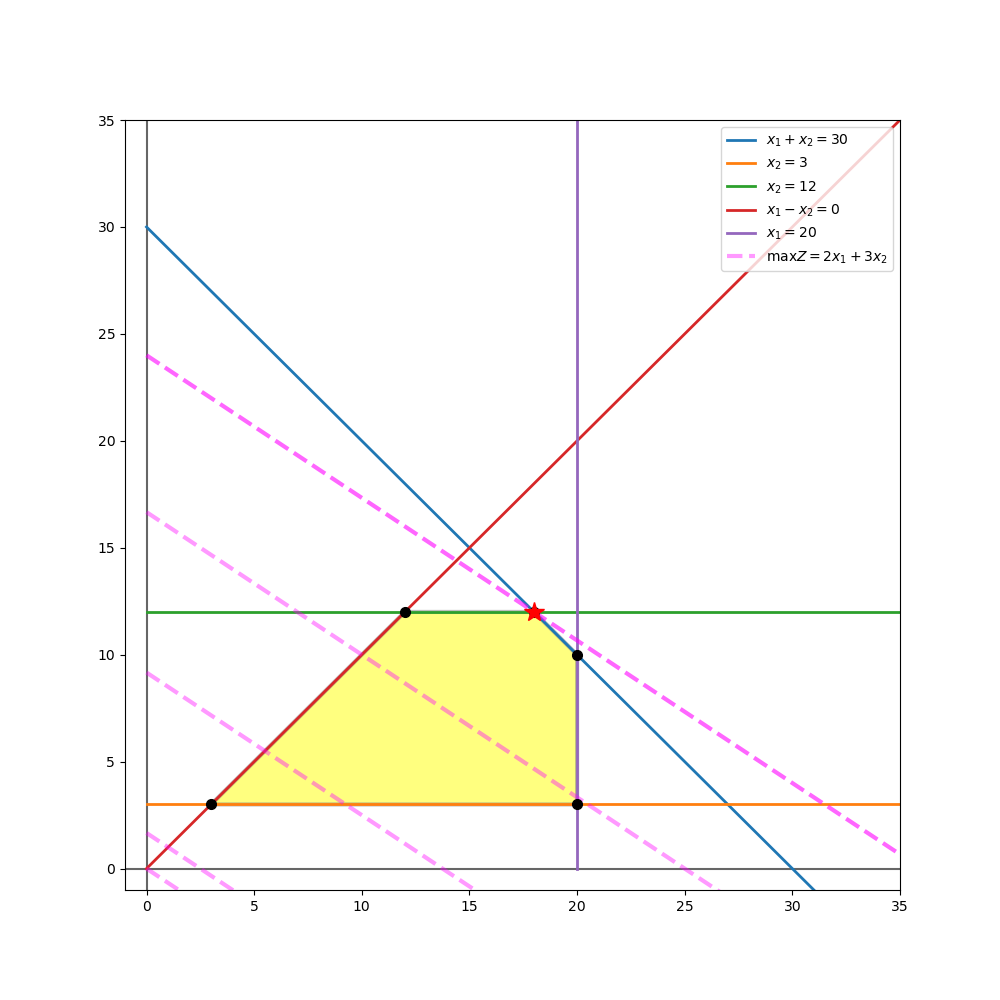
\includegraphics[scale=0.4]{fig_simplex-artificial-variables.png}
    %   \par}
    % \end{onlyenv}
\end{frame}


\begin{frame}{Método de Penalización. Ejemplo.}{}
  {\centering
      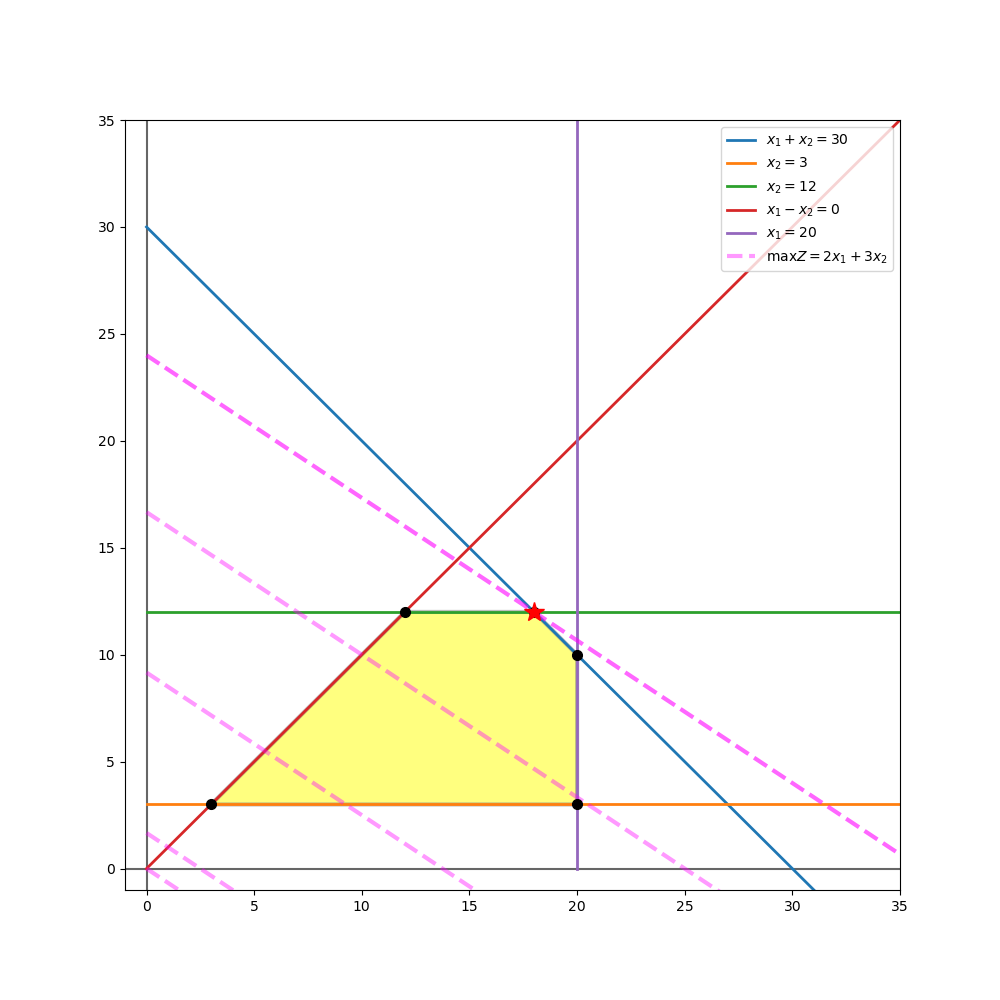
\includegraphics[scale=0.32]{fig_simplex-artificial-variables.png}
      \par}
\end{frame}

\begin{frame}{The Two-Phase Method}
  In the preceding  section we observed that it was frequently necessary to add artificial variables to the constraints to obtain an initial basic feasible solution to an L.P. problem. If the problem is to be solved, \alert{the artificial variables must be driven to zero}. The two-phase method is another method to handle these artificial variables. Here \alert{the L.P. problem is solved in two phases}.  
\end{frame}


\begin{frame}{The Two-Phase Method. Phase I}
  \begin{itemize} \justifying \parskip3mm
  \item<only@1> An artificial objective function $(W)$ is created which is \alert{the sum of all the artificial variables}.
  \item<only@1,2> \alert{The new objective function is then minimized}, subject to the \alert{constraints of the given (original) problem} using the simplex method. At the end of the phase I, three cases arise:
    \begin{enumerate} \justifying
    \item<only@2> If the \alert{minimum $W > 0$}, and at least one artificial variable appears in the basis at a positive level,  \alert{the given problem has no feasible solution} and the procedure terminates.
    \item<only@2> If the minimum value of \alert{$W = 0$, and no artificial variable appears in the basis}, then \alert{a basic feasible solution to the given problem is obtained}.
    \item<only@2> \alert{If the mimimum value of $W = 0$ and one or more artificial variables appear in the basis at zero level}, then a feasible solution to the original problem is obtained. However, \alert{we must take care of this artificial variable and see that it never becomres positive during phase II computations}. Zero cost coefficients is assigned to this artificial variable and it is retained in the initial table of phase II.
    \end{enumerate}
  \end{itemize}
\end{frame}


\begin{frame}{The Two-Phase Method. Phase II}
  When phase I results in case 2 and 3, we go on to phase II to find optimum solution to the given L.P. problem. The basic feasible solution found at the end of phase I is now used as a starting solution for the original problem. In other words, \alert{the final table of phase I becomes the starting table of phase II in which the artificial (auxiliary) objective function is replaced by the original objective function. The simplex method is then applied to arrive at the optimum solution}. Artificial variables which do not appear in the basis may be deleted.
\end{frame}


\begin{frame}{The Two Phase Method. A First Example}
  Use the two-phase method simplex method to

  \[\max Z = 5x_1 + 3x_2\]

  {\centering
    s.t.

  \sysdelim..%
  \sysalign{r,r}%
  \systeme[x_1x_2]%
  {%
    2x_1 + x_2 \leq 1,
    x_1 + 4x_2 \geq 6
  }

  $x_1, x_2 \geq 0$
\par}
\end{frame}

\begin{frame}{The Two-Phase Method. A First Example. Phase I}

  \begin{block}<only@1>{Step 1. Set up the Problem in the Standard Form} \justifying
    The original objective function $Z = 5x_1 + 3x_2$ is temporarily set aside during the phase I solution. The given constraints, after the introduction of slack, surplus and artificial variables take de the form:


    s.t.

    \sysdelim..%
    \sysalign{r,r}%
    \systeme[x_1x_2s_1s_2A_1]{%
      2x_1 + x_2 + s_1 = 1,
      x_1 + 4x_2 - s_2 + A_1 = 6
    }

    \vspace{5mm}
    The new objective function is \[ \min W = A \]
    
  \end{block}
  
  \begin{block}<only@2>{Step 1. Set up the Problem in the Standard Form.} \justifying

    The simplex method requires that a variable which appears in one equation appear in all the equations. This is done by proper placemente of a zero coefficient. Thus the problem for phase I in standard form becomes

   $\min W = 0x_1 + 0x_2 + 0s_1 + 0s_2 + A_1$ 

   s.t.

   \sysdelim..%
   \sysalign{r,r}%
    \systeme[x_1x_2s_1s_2A_1]{%
      2x_1 + x_2 + s_1  = 1,
      x_1 + 4x_2  - s_2 + A_1 = 6
    }
    
    $x_1, x_2, s_1, s_2, A_1 \geq 0$
    
  \end{block}

  \begin{block}<only@3>{Step 2. Find an Initial Basic Feasible Solution}

    {\centering
      \begin{tabular}{rcrrrrrrrl}
        \toprule
        &$c_j$&0&0&0&0&1&&&\\
        $c_B$&Basis&$x_1$&\cellcolor{yellow}$x_2$&$s_1$&$s_2$&$A_1$&$b$&$\theta$&\\
        \midrule
        0&\cellcolor{yellow}$s_1$&2&\cellcolor{orange}1&0&1&0&1&1&\textrightarrow\\
        1&$A_1$&1&4&-1&0&1&6&3/2&\\
        \midrule
        &$Z_j$&1&4&-1&0&1&\cellcolor{red!30}6&&\\
        &$c_j -Z_j$&-1&-4&1&0&0&&&\\
        \toprule
        &&&\textuparrow&&&&&&\\
      \end{tabular}
    \par}
    
\end{block}

\begin{block}<only@3>{Step 3. Perform Optimality Test} \justifying
  Since $c_j - Z_j$ is negative under some columns (minimization problem), the preceding table is not optimal.
\end{block}

\begin{block}<only@4>{Step 4. Iterate Towards An Optimal Solution.} \justifying
    {\centering
      \begin{tabular}{rcrrrrrrrl}
        \toprule
        &$c_j$&0&0&0&0&1&&&\\
        $c_B$&Basis&$x_1$&$x_2$&$s_1$&$s_2$&$A_1$&$b$&&\\
        \midrule
        0&$x_2$&2&1&0&1&0&1&&\\
        
        1&\cellcolor{yellow}$A_1$&-7&0&-1&-4&1&\cellcolor{yellow}2&&\\
        \midrule
        &$Z_j$&-7&0&-1&-4&1&\cellcolor{red!30}2&&\\
        &$c_j -Z_j$&\cellcolor{blue!30}7&\cellcolor{blue!30}0&\cellcolor{blue!30}1&\cellcolor{blue!30}4&\cellcolor{blue!30}0&&&\\
        \toprule
      \end{tabular}
      \par}
    Optimal basic feasible solution for phase I problem. 
  \end{block}

  \only<4>{%
    $c_j - Z_j$ is either positive or zero under all columns, an optimal basic feasible solution to the auxiliary L.P.P. has been obtained.

    However, since $W=A=2 (> 0)$ and artificial variable $A_1$ appears in the basis at a positive level ($A_1 = 2$), \alert{the given problem does not posses a feasible solution and the procedure stops}.%
  }
\end{frame}



\begin{frame}{The Two-Phase Method. An example.}{}
  \begin{onlyenv}<1>
    \begin{columns}[t]
      \column{0.3\textwidth}

\[        \max Z = 2x_1 + 3x_2  \]

{\centering
  subject to

  \sysdelim..\sysalign{r,r}%
  \systeme[x_1x_2]%
  {
    x_1 + x_2  \leq 30,
    x_2  \geq 3,
    x_2  \leq 12,
    -x_1 + x_2  \leq 0,
    x_1   \leq 20
  }

  \vspace{5mm}
  $x_1, x_2  \geq 0$
  \par}
        
      \column{0.6\textwidth}
      \[ \max Z = 2x_1 + 3x_2\]
      {\centering
        s.t.

      \sysdelim..%
      \sysalign{r,r}%
      \systeme[x_1x_2s_1s_2s_3s_4s_5]{%
        x_1 + x_2 + s_1 = 30,
        x_2  - s_2  = 3,
        x_2  + s_3 = 12,
        -x_1 + x_2 + s_4  =  0,
        x_1  + s_5 = 20 }

      \vspace{5mm}
      $x_1, x_2, s_1, s_2, s_3, s_4, s_5  \geq 0$
    \par} 
    \end{columns}
  \end{onlyenv}

  \begin{onlyenv}<2>
    \[ \min W = 0x_1 + 0x_2 +0s_1 - 0s_2 + 0s_3 + 0s_4 + 0s_5 + A_2 \]

    {\centering
      s.t.
      
    \sysdelim..\sysalign{r,r}%
    \systeme[x_1x_2s_1s_2s_3s_4s_5A_2]%
    {%
      x_1 + x_2 + s_1 = 30,
      x_2  - s_2  + A_2 = 3,
      x_2  + s_3 = 12,
      -x_1 + x_2 + s_4  =  0,
      x_1  + s_5 = 20 }

    $x_1, x_2, s_1, s_2, s_3, s_4, s_5, A_2  \geq 0$
  \par}
  \end{onlyenv}
\end{frame}

\begin{frame}{The Two-Phase Method. An example.}{}
  \begin{onlyenv}<1>
    \[ \min W = A_2 \]

    {\centering
    subject to

    \sysalign{r,r}
    \sysdelim..
    \systeme[x_1x_2s_1s_2s_3s_4s_5A_2]{%
      x_1 + x_2 + s_1 = 30,
      x_2  - s_2  + A_2 = 3,
      x_2  + s_3 = 12,
      -x_1 + x_2 + s_4  =  0,
      x_1  + s_5 = 20 }

    \vspace{5mm}
    $x_1, x_2, s_1, s_2, s_3, s_4, s_5, A_2  \geq 0$
    \par}
  \end{onlyenv}
\end{frame}

\begin{frame}{The Two-Phase Method. An example. Phase I.}{}
  {\centering
    \scalebox{1}{%
      \begin{tabular}{rc|llllllll|rr}
        & $\min$ & 0 & 0 & 0 & 1 & 0 & 0 & 0 & 0 &  &  \\
        \midrule
        $\mathbf{C_b}$ & \textbf{basis} & $x_1$ & $x_2$ & $s_1$ & $A_2$ & $s_3$ & $s_4$ & $s_5$ & $s_2$ & RHS & ratios \\
        \midrule
        \only<1>{
        0 & $s_1$ & 1 & 1 & 1 & 0 & 0 & 0 & 0 & 0 & 30 & 30 \\
        1 & $A_2$ & 0 & 1 & 0 & 1 & 0 & 0 & 0 & -1 & 3 & 3 \\
        0 & $s_3$ & 0 & 1 & 0 & 0 & 1 & 0 & 0 & 0 & 12 & 12 \\
        0 & $s_4$ & -1 & \cellcolor{yellow}1 & 0 & 0 & 0 & 1 & 0 & 0 & 0 & 0 \\
        0 & $s_5$ & 1 & 0 & 0 & 0 & 0 & 0 & 1 & 0 & 20 & \#DIV/0! \\
        \midrule
        Iter & $Z_j$ & 0 & 1 & 0 & 1 & 0 & 0 & 0 & -1 & 3 &  \\
        1& $c_j - Z_j$ & 0 & -1 & 0 & 0 & 0 & 0 & 0 & 1 &  & 
                                                             }
                                                             \only<2>{%
                                                             0 & $s_1$ & 2 & 0 & 1 & 0 & 0 & -1 & 0 & 0 & 30 &  \\
        1 & $A_2$ & 1 & 0 & 0 & 1 & 0 & -1 & 0 & -1 & 3 &  \\
        0 & $s_3$ & 1 & 0 & 0 & 0 & 1 & -1 & 0 & 0 & 12 &  \\
        0 & $x_2$ & -1 & \cellcolor{yellow}1 & 0 & 0 & 0 & 1 & 0 & 0 & 0 &  \\
        0 & $s_5$ & 1 & 0 & 0 & 0 & 0 & 0 & 1 & 0 & 20 &  \\
        \midrule
        Iter& $Z_j$ & 1 & 0 & 0 & 1 & 0 & -1 & 0 & -1 & 3 &  \\
        1& $c_j - Z_j$ & -1 & 0 & 0 & 0 & 0 & 1 & 0 & 1 &&                                                  
                                                           }
                                                           \only<3>{
                                                           0 & $s_1$ & 2 & 0 & 1 & 0 & 0 & -1 & 0 & 0 & 30 & 15 \\
        1 & $A_2$ & \cellcolor{yellow}1 & 0 & 0 & 1 & 0 & -1 & 0 & -1 & 3 & 3 \\
        0 & $s_3$ & 1 & 0 & 0 & 0 & 1 & -1 & 0 & 0 & 12 & 12 \\
        0 & $x_2$ & -1 & 1 & 0 & 0 & 0 & 1 & 0 & 0 & 0 & -0 \\
        0 & $s_5$ & 1 & 0 & 0 & 0 & 0 & 0 & 1 & 0 & 20 & 20 \\
        \midrule
        Iter& $Z_j $& 1 & 0 & 0 & 1 & 0 & -1 & 0 & -1 & 3 &  \\
        2& $c_j - Z_j$ & -1 & 0 & 0 & 0 & 0 & 1 & 0 & 1 &  &
                                                             }
                                                             \only<4>{%
                                                             0 & $s_1$ & 0 & 0 & 1 & -2 & 0 & 1 & 0 & 2 & 24 & 15 \\
        0 & $x_1$ & \cellcolor{yellow}1 & 0 & 0 & 1 & 0 & -1 & 0 & -1 & 3 & 3 \\
        0 & $s_3$ & 0 & 0 & 0 & -1 & 1 & 0 & 0 & 1 & 9 & 12 \\
        0 & $x_2$ & 0 & 1 & 0 & 1 & 0 & 0 & 0 & -1 & 3 &  \\
        0 & $s_5$ & 0 & 0 & 0 & -1 & 0 & 1 & 1 & 1 & 17 & 20 \\
        \midrule
        Iter& $Z_j$ & 0 & 0 & 0 & 0 & 0 & 0 & 0 & 0 & 0 &  \\
        2& $c_j - Z_j$ & 0 & 0 & 0 & 1 & 0 & 0 & 0 & 0 &  & 
                                                            }
      \end{tabular}
    } % scalebox
    \par}
\end{frame}

\begin{frame}{The Two-Phase Method. An example. Phase II.}{}
Fase II
  
  {\centering
    \begin{tabular}{rl|rrrrrrr|rr}
      & $\max$ & 2 & 3 & 0 & 0 & 0 & 0 & 0 &  &  \\
      \midrule
      $\mathbf{C_b}$ & \textbf{basis} & $x_1$ & $x_2$ & $s_1$ & $s_3$ & $s_4$ & $s_5$ & $s_2$ & RHS & ratios \\
      \midrule
      % ==============================
      \only<1>{
      0 & $s_1$ & 0 & 0 & 1 & 0 & 1 & 0 & 2 & 24 & 12 \\
      2 & $x_1$ & 1 & 0 & 0 & 0 & -1 & 0 & -1 & 3 & -3 \\
      0 & $s_3$ & 0 & 0 & 0 & 1 & 0 & 0 & \cellcolor{yellow}1 & 9 & 9 \\
      3 & $x_2$ & 0 & 1 & 0 & 0 & 0 & 0 & -1 & 3 & -3 \\
      0 & $s_5$ & 0 & 0 & 0 & 0 & 1 & 1 & 1 & 17 & 17 \\
      \midrule
      Iter& $Z_j$ & 2 & 3 & 0 & 0 & -2 & 0 & -5 & 15 &  \\
      3& $c_j - Z_j$ & 0 & 0 & 0 & 0 & 2 & 0 & 5 &  &    
                                                      }% only
                                                      %%% 
                                                      \only<2>{
                                                      0 & $s_1$ & 0 & 0 & 1 & -2 & 1 & 0 & 0 & 6 &\\
      2 & $x_1$ & 1 & 0 & 0 & 1 & -1 & 0 & 0 & 12 &\\
      0 & $s_2$ & 0 & 0 & 0 & 1 & 0 & 0 & \cellcolor{yellow}1 & 9 &\\
      3 & $x_2$ & 0 & 1 & 0 & 1 & 0 & 0 & 0 & 12 &\\
      0 & $s_5$ & 0 & 0 & 0 & -1 & 1 & 1 & 0 & 8 &\\\midrule
      Iter & $Z_j$ & 2 & 3 & 0 & 5 & -2 & 0 & 0 & 60 &\\
      3 & $c_j - Z_j$ & 0 & 0 & 0 & -5 & 2 & 0 & 0 &&
                                                      }%only
                                                      % ------
                                                      \only<3>{%
                                                      0 & $s_1$ & 0 & 0 & 1 & -2 & \cellcolor{yellow}1 & 0 & 0 & 6 & 6 \\
      2 & $x_1$ & 1 & 0 & 0 & 1 & -1 & 0 & 0 & 12 & -12 \\
      0 & $s_2$ & 0 & 0 & 0 & 1 & 0 & 0 & 1 & 9 & \#DIV/0! \\
      3 & $x_2$ & 0 & 1 & 0 & 1 & 0 & 0 & 0 & 12 & \#DIV/0! \\
      0 & $s_5$ & 0 & 0 & 0 & -1 & 1 & 1 & 0 & 8 & 8 \\ \midrule
      Iter & $Z_j$ & 2 & 3 & 0 & 5 & -2 & 0 & 0 & 60 &  \\
      4 & $c_j - Z_j$ & 0 & 0 & 0 & -5 & 2 & 0 & 0 &  &
                                                        } %
                                                        \only<4>{
                                                        0 & $s_4$ & 0 & 0 & 1 & -2 & \cellcolor{yellow}1 & 0 & 0 & 6 &  \\
      2 & $x_1$ & 1 & 0 & 1 & -1 & 0 & 0 & 0 & 18 &  \\
      0 & $s_2$ & 0 & 0 & 0 & 1 & 0 & 0 & 1 & 9 &  \\
      3 & $x_2$ & 0 & 1 & 0 & 1 & 0 & 0 & 0 & 12 &  \\
      0 & $s_5$ & 0 & 0 & -1 & 1 & 0 & 1 & 0 & 2 &  \\\midrule
      Iter & $Z_j$ & 2 & 3 & 2 & 1 & 0 & 0 & 0 & 72 &  \\
      4 & $c_j - Z_j$ & 0 & 0 & -2 & -1 & 0 & 0 & 0 & \textbf{END} & %//
                                                                     }
                                                                     % =================================
    \end{tabular}
    \par}
\end{frame}

\begin{frameExample}{Diet Problem}{}
  % EXAMPLE 2.6-2 {Diet Problem} Gupta
  \begin{onlyenv}<1>
      La persona quiere decidir los componentes de una dieta que cumpla con sus requerimientos diarios de proteínas, grasas y carbohidratos al costo mínimo. La elección debe hacerse a partir de cuatro tipos diferentes de alimentos. Los rendimientos por unidad de estos alimentos se dan en la tabla siguiente. Formule un modelo de programación lineal para el problema y resuelva por método simplex.


  {\centering
    \scalebox{0.7}{
      \begin{tabular}{ccccc}
        \toprule
        Comida        & Proteinas & Grasas & Carbohidratos & Costo \$ \\
        \midrule
        1             & 3         & 2      & 6             & 45    \\
        2             & 4         & 2      & 4             & 40    \\
        3             & 8         & 7      & 7             & 85    \\
        4             & 6         & 5      & 4             & 65    \\
        \midrule
        Requerimiento &           &        &               &       \\
        Mínimo        & 800       & 200    & 700           &\\
        \bottomrule
      \end{tabular}
    } % scalebox
    \par}    
\end{onlyenv}

  \begin{onlyenv}<2>
    \[ \min Z = 45x_1 + 40x_2 + 85x_3 + 65x_4   \]

    {\centering
      s.t.  %
      
    \scalebox{0.95}{%
      % \syssignspace{3pt}
      \sysdelim..\sysalign{r,r}%
      \systeme[x_1x_2x_3x_4]%
      {%
        3x_1 + 4x_2 + 8x_3 + 6x_4 \geq  800,
        2x_1 + 2x_2 + 7x_3 + 5x_4 \geq 200,
        6x_1  +4x_2 + 7x_3 + 4x_4 \geq 700%
      }
    }% scalebox

    $x_1, x_2, x_3, x_4 \geq 0$
  \par}
  \end{onlyenv}
  
  \begin{onlyenv}<3>
    \[ \min W = 0x_1 + 0x_2 + 0x_3 + 0x_4 - 0s_1 - 0s_2 - 0s_3  + A_1 + A_2 + A_3 \]

    {\centering
      s.t.  %
      
    \scalebox{0.95}{%
      \sysdelim..\sysalign{r,r}%
      \systeme[x_1x_2x_3x_4s_1s_2s_3A_1A_2A_3]{%
        3x_1 + 4x_2 + 8x_3 + 6x_4 - s_1 + A_1 = 800,
        2x_1 + 2x_2 + 7x_3 + 5x_4 - s_2 + A_2 = 200,
        6x_1  +4x_2 + 7x_3 + 4x_4 - s_3 + A_3 = 700, }
    }% scalebox

    $x_1, x_2, x_3, x_4, s_1, s_2, s_3, A_1, A_2, A_3  \geq 0$
  \par}
  \end{onlyenv}
  \begin{onlyenv}<4>
    \[ \min W = A_1 + A_2 + A_3 \]

    {\centering
      s.t.

      
    \scalebox{0.95}{%
      \sysdelim..\sysalign{r,r}%
      \systeme[x_1x_2x_3x_4s_1s_2s_3A_1A_2A_3]{%
        3x_1 + 4x_2 + 8x_3 + 6x_4 - s_1 + A_1 = 800,
        2x_1 + 2x_2 + 7x_3 + 5x_4 - s_2 + A_2 = 200,
        6x_1  +4x_2 + 7x_3 + 4x_4 - s_3 + A_3 = 700, }
    }% scalebox

    $x_1, x_2, x_3, x_4, s_1, s_2, s_3, A_1, A_2, A_3  \geq 0$
    \par}
  \end{onlyenv}

\end{frameExample}






%%% Local Variables:
%%% mode: latex
%%% TeX-master: "slides"
%%% End:
